\section{Background}\label{sec:problem}
Consider a swarm $\mathcal{N}$ that contains $N$ robots labelled $i\in\left\{1,...,N\right\}$. We model the swarm as a directed sensing graph $\mathcal{G}=\left(\mathcal{V},\mathcal{E}\right)$, where vertex set $\mathcal{V} = \left\{1,..., N\right\}$ represents the robots, and edge set $\mathcal{E}\subseteq\mathcal{V}\times \mathcal{V}$ contains the pairs of robots $\left(i, j\right)\in\mathcal{E}$ for which robot $i$ can sense robot $j$. We denote $\mathcal{N}_i=\left\{j\in\mathcal{V}|\left(i,j\right)\in\mathcal{E}\right\}\subset\mathcal{V}$ as the set of $N_i$ neighbours of a robot $i$ in $\mathcal{G}$.

In our study, the dynamics of the robots are represented in discrete time. Denote $p_i(k),v_i(k),u_i(k)\in\mathbb{R}^3$ respectively be the position, velocity and control input of the robot $i$ at the time $t(k) = k\tau$, where $\tau$ is the time step. The robots in the swarm are homogeneous with a body radius $r$. Each robot $i$ is equipped with an inertial measurement unit (IMU) to determine its position and orientation to a desired direction, a range sensor, and a wireless ad-hoc network module to carry out peer-to-peer communication with other robots. In this work, the communication delay between each pair of robots is negligible~\cite{AlonsoMora2018,9527169}. The local sensor is equipped on each robot to provide a $360^\circ$ field of view of the surrounding environment and can scan a maximum area $S_s$ within radius $r_s$, as shown in Fig.~\ref{fig:model}. A set $\mathcal{M}_i(k)=\left\{m\right\}$ represents the observed obstacle points at time $t(k)$.
\begin{figure}
    \centering
    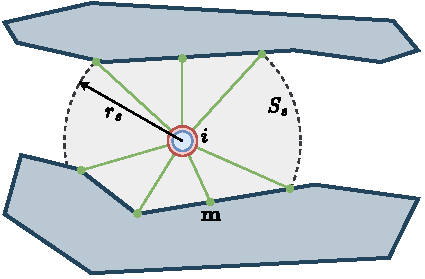
\includegraphics[width=0.48\textwidth]{paper3/images/model.pdf}
    \caption{Illustration of a robot with a local range sensor. Each robot is equipped with a local sensor with sensing area $S_s$ (dashed gray circle) being a circular disk with radius $r_s$. The set $\mathcal{M}_i=\{m\}$ (green) is the observed point cloud data.}
    \label{fig:model}
\end{figure}

According to~\cite{Soria2021}, assuming that every robot in the swarm obeys a discrete linear system, given by
\begin{equation}
    x_i(k+1)=A_ix_i(k) + B_iu_i(k)
\end{equation}
where $A_i$ and $B_i$ are constant matrices. We consider the system to represent a robot with an underlying acceleration controller. The input $u_i$ is an acceleration command, and the state $x_i=\left[p_i;v_i\right]\in\mathbb{R}^6$ is a vector containing the position and velocity. The velocities and accelerations of the robots are bounded by constant vectors, i.e. $v_\text{min}\leq v_i(k)\leq v_\text{max}$ and $u_\text{min}\leq u_i(k)\leq u_\text{max}$.